\documentclass{standalone}
\usepackage{tikz}
\usepackage{pgfplots}
\begin{document}
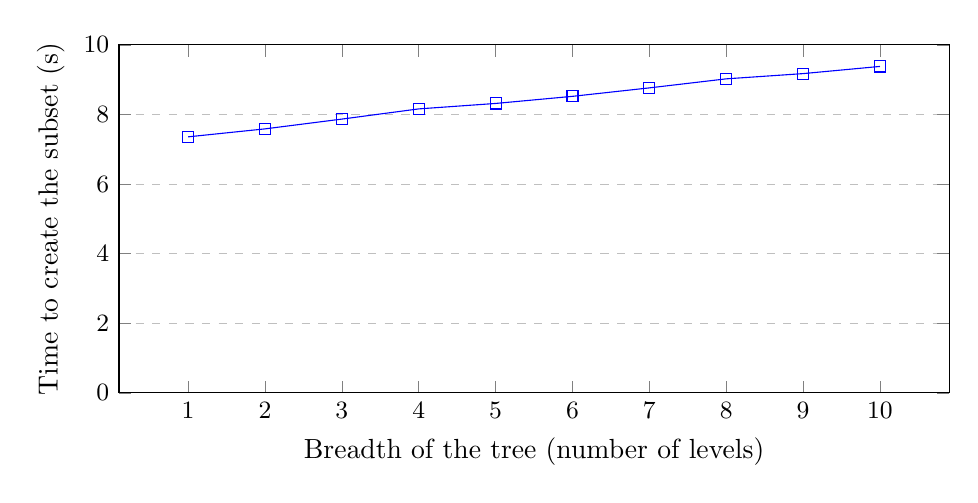
\begin{tikzpicture}
    \begin{axis}[
            title={},
            xlabel={Breadth of the tree (number of levels)},
            ylabel={Time to create the subset (s)},
            ymin=0, ymax=10,
            xtick=data,
            height=6cm,
            width=\textwidth,
            legend pos=north west,
            ymajorgrids=true,
            grid style=dashed,
            tick align=inside,
            every tick label/.append style={font=\small}
        ]
        \addplot[
            color=blue,
            mark=square,
        ]
        coordinates {
                (1,7.357845308)
                (2,7.586814884)
                (3,7.868225595)
                (4,8.161074051)
                (5,8.317615008)
                (6,8.522139853)
                (7,8.765099077)
                (8,9.024716349)
                (9,9.175310546)
                (10,9.381863443)
            };
    \end{axis}
\end{tikzpicture}
\end{document}